% This is an included file. See the master file for more information.
%
% When editing this file:
%
%    1. To change formatting, appearance, or style, please edit openmp.sty.
%
%    2. Custom commands and macros are defined in openmp.sty.
%
%    3. Be kind to other editors -- keep a consistent style by copying-and-pasting to
%       create new content.
%
%    4. We use semantic markup, e.g. (see openmp.sty for a full list):
%         \code{}     % for bold monospace keywords, code, operators, etc.
%         \plc{}      % for italic placeholder names, grammar, etc.
%
%    5. There are environments that provide special formatting, e.g. language bars.
%       Please use them whereever appropriate.  Examples are:
%
%         \begin{fortranspecific}
%         This is text that appears enclosed in blue language bars for Fortran.
%         \end{fortranspecific}
%
%         \begin{note}
%         This is a note.  The "Note -- " header appears automatically.
%         \end{note}
%
%    6. Other recommendations:
%         Use the convenience macros defined in openmp.sty for the minor headers
%         such as Comments, Syntax, etc.
%
%         To keep items together on the same page, prefer the use of
%         \begin{samepage}.... Avoid \parbox for text blocks as it interrupts line numbering.
%         When possible, avoid \filbreak, \pagebreak, \newpage, \clearpage unless that's
%         what you mean. Use \needspace{} cautiously for troublesome paragraphs.
%
%         Avoid absolute lengths and measures in this file; use relative units when possible.
%         Vertical space can be relative to \baselineskip or ex units. Horizontal space
%         can be relative to \linewidth or em units.
%
%         Prefer \emph{} to italicize terminology, e.g.:
%             This is a \emph{definition}, not a placeholder.
%             This is a \plc{var-name}.
%


\chapter{OMPT Interface}
\label{sec:OMPT Interface}
\label{chap:OMPT Interface}
\label{sec:ompt-overview}

This chapter describes OMPT, which is an interface for \emph{first-party}
tools. \emph{First-party} tools are linked or loaded directly into the OpenMP 
program. OMPT defines mechanisms to initialize a tool, to examine OpenMP state 
associated with an OpenMP thread, to interpret the call stack of an OpenMP 
thread, to receive notification about OpenMP \emph{events}, to trace activity 
on OpenMP target devices, to assess implementation-dependent details of an 
OpenMP implementation (such as supported states and mutual exclusion 
implementations), and to control a tool from an OpenMP application.

\section{OMPT Interfaces Definitions}
\index{tool interfaces definitions}
\index{tools header files}
\label{sec:OMPT Interfaces Definitions}

\begin{ccppspecific}
A compliant implementation must supply a set of definitions for the OMPT runtime
entry points, OMPT callback signatures, and the special data types of
their parameters and return values. These definitions, which are listed throughout
this chapter, and their associated declarations shall be provided in a header file
named \code{omp-tools.h}. In addition, the set of definitions may specify other
implementation-specific values.

The \code{ompt_start_tool} function is an external function with \code{C} linkage.
\end{ccppspecific}

\section{Activating a First-Party Tool}
\label{sec:ompt-initialization}

To activate a tool, an OpenMP implementation first determines whether 
the tool should be initialized. If so, the OpenMP implementation invokes 
the initializer of the tool, which enables the tool to prepare to monitor 
execution on the host. The tool may then also arrange to monitor computation 
that executes on target devices. This section explains how the tool and an
OpenMP implementation interact to accomplish these tasks.

\subsubsection{\hcode{ompt_start_tool}}
\label{sec:ompt_start_tool}

\summary
If a tool wants to use the OMPT interface provided by an OpenMP implementation,
the tool must implement the function \code{ompt_start_tool} to announce its interest.

\format

\begin{cspecific}
\begin{omptOther}
ompt_start_tool_result_t *ompt_start_tool(
  unsigned int \plc{omp_version},
  const char *\plc{runtime_version}
);
\end{omptOther}
\end{cspecific}


\descr
For a tool to use the OMPT interface provided by an OpenMP implementation,
the tool must define a globally-visible implementation of the
function \code{ompt_start_tool}.

A tool may indicate its intent to use the OMPT interface provided
by an OpenMP implementation by having
\code{ompt_start_tool} return a non-null pointer to an
\code{ompt_start_tool_result_t} structure, which contains pointers to
tool initialization and finalization callbacks along with
a tool data word that an OpenMP implementation must pass by reference
to these callbacks.

A tool may use its argument \plc{omp_version} to determine
whether it is compatible with the OMPT interface provided by an OpenMP
implementation.

If a tool implements \code{ompt_start_tool} but has no interest in using
the OMPT interface in a particular execution,
\code{ompt_start_tool} should return \code{NULL}.

\argdesc

The argument \plc{omp_version}
is the value of the \code{_OPENMP} version macro
associated with the OpenMP API implementation. This value
identifies the OpenMP API version supported by an OpenMP implementation,
which specifies the version of the OMPT interface that it supports.

The argument \plc{runtime_version}
is a version string that unambiguously identifies the OpenMP implementation.

\constraints

The argument \plc{runtime_version} must be
an immutable string that is defined for the lifetime of a program
execution.

\effect
If a tool returns a non-null pointer to an
\code{ompt_start_tool_result_t} structure,
an OpenMP implementation will call the tool initializer specified by the
\plc{initialize} field in this structure before
beginning execution of any OpenMP construct
or completing execution of any environment routine invocation; the
OpenMP implementation will call the tool finalizer specified by the
\plc{finalize} field in this structure when the OpenMP
implementation shuts down.



\crossreferences
\begin{itemize}
    \item \code{ompt_start_tool_result_t}, see
     \specref{sec:ompt_start_tool_result_t}.
\end{itemize}





\subsection{Determining Whether a First-Party Tool Should be Initialized}
\label{sec:ompt-check-tool}

\begin{figure}[h]
  \centering
  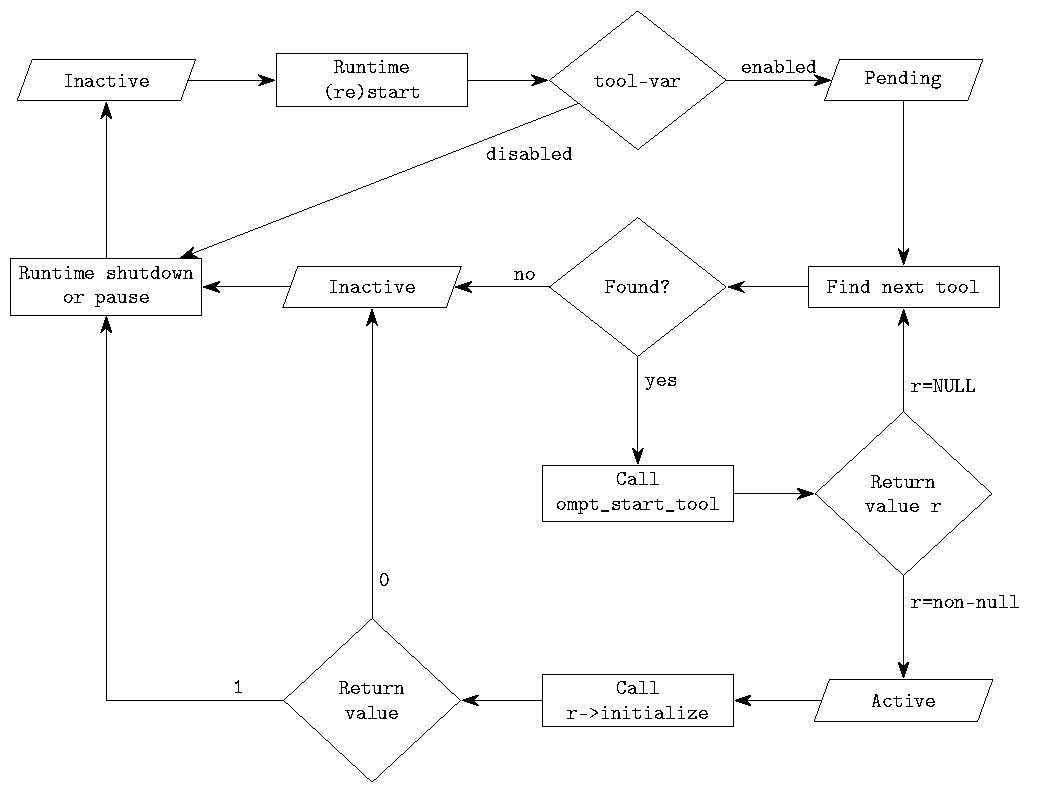
\includegraphics[width=.9\linewidth]{tool_support/ompt_flow_chart.pdf}
  \caption{First-Party Tool Activation Flow Chart}
  \label{fig:ompt_diagram}
\end{figure}

An OpenMP implementation examines the \plc{tool-var} ICV as one of its first 
initialization steps. If the value of \plc{tool-var} is \plc{disabled}, the 
initialization continues without a check for the presence of a tool and 
the functionality of the OMPT interface will be unavailable as the program 
executes. In this case, the OMPT interface state remains \emph{inactive}.

Otherwise, the OMPT interface state changes to \emph{pending} and the 
OpenMP implementation activates any first-party tool that it finds. A 
tool can provide a definition of \code{ompt_start_tool} to an OpenMP 
implementation in three ways:

\begin{itemize}
\item By statically-linking its definition of \code{ompt_start_tool} into an
      OpenMP application;
\item By introducing a dynamically-linked library that includes its definition
      of \code{ompt_start_tool} into the application's address space; or
\item By providing, in the \plc{tool-libraries-var} ICV, the name of a 
      dynamically-linked library that is appropriate for the architecture and 
      operating system used by the application and that includes a
      definition of \code{ompt_start_tool}.
\end{itemize}

If the value of \plc{tool-var} is \plc{enabled}, the OpenMP implementation 
must check if a tool has provided an implementation of \code{ompt_start_tool}. 
The OpenMP implementation first checks if a tool-provided implementation of 
\code{ompt_start_tool} is available in the address space, either 
statically-linked into the application or in a dynamically-linked library 
loaded in the address space. If multiple implementations of 
\code{ompt_start_tool} are available, the OpenMP implementation will use 
the first tool-provided implementation of \code{ompt_start_tool} that it finds.

If the implementation does not find a tool-provided implementation of 
\code{ompt_start_tool} in the address space, it consults the 
\plc{tool-libraries-var} ICV, which contains a (possibly empty) list of 
dynamically-linked libraries. As  described in detail in 
\specref{sec:OMP_TOOL_LIBRARIES}, the libraries in \plc{tool-libraries-var} 
are then searched for the first usable implementation of 
\code{ompt_start_tool} that one of the libraries in the list provides.

If the implementation finds a tool-provided definition of 
\code{ompt_start_tool}, it invokes that method; if a \code{NULL} pointer 
is returned, the OMPT interface state remains \emph{pending} and the 
implementation continues to look for implementations of \code{ompt_start_tool};
otherwise a non-null pointer to an \code{ompt_start_tool_result_t} 
structure is returned, the OMPT interface state changes to \emph{active} 
and the OpenMP implementation makes the OMPT interface available as the 
program executes. In this case, as the OpenMP implementation completes its 
initialization, it initializes the OMPT interface.

If no tool can be found, the OMPT interface state changes to \emph{inactive}.

\crossreferences
\begin{itemize}
\item \plc{tool-libraries-var} ICV, 
see \specref{sec:Internal Control Variables}.

\item \plc{tool-var} ICV, see \specref{sec:Internal Control Variables}.

\item \code{ompt_start_tool} function, see \specref{sec:ompt_start_tool}.

\item \code{ompt_start_tool_result_t} type, 
see \specref{sec:ompt_start_tool_result_t}.
\end{itemize}

\subsection{Initializing a First-Party Tool}
\index{tool initialization}
\label{sec:tool-initialize}

To initialize the OMPT interface, the OpenMP implementation invokes the tool 
initializer that is specified in the \code{ompt_start_tool_result_t} structure
that is indicated by the non-null pointer that \code{ompt_start_tool} returns.
The initializer is invoked prior to the occurrence of any OpenMP \emph{event}.

A tool initializer, described in \specref{sec:ompt_initialize_t}, uses the 
function specified in its \plc{lookup} argument to look up pointers to OMPT 
interface runtime entry points that the OpenMP implementation provides; this 
process is described in \specref{sec:ompt-bind}. Typically, a tool initializer
obtains a pointer to the  \code{ompt_set_callback} runtime entry point with 
type signature \code{ompt_set_callback_t} and then uses this runtime entry 
point to register tool callbacks for OpenMP events, as described in 
\specref{sec:ompt-register-callbacks}.

A tool initializer may use the \code{ompt_enumerate_states} runtime entry 
point, which has type signature \code{ompt_enumerate_states_t}, to determine 
the thread states that an OpenMP implementation employs. Similarly, it may
use the \code{ompt_enumerate_mutex_impls} runtime entry point, which has 
type signature \code{ompt_enumerate_mutex_impls_t}, to determine the mutual
exclusion implementations that the OpenMP implementation employs.

If a tool initializer returns a non-zero value, the OMPT interface state
remains \emph{active} for the execution; otherwise, the OMPT interface state 
changes to \emph{inactive}.

\crossreferences
\begin{itemize}
\item \code{ompt_start_tool} function, see \specref{sec:ompt_start_tool}.

\item \code{ompt_start_tool_result_t} type, see
  \specref{sec:ompt_start_tool_result_t}.

\item \code{ompt_initialize_t} type, see \specref{sec:ompt_initialize_t}.

\item \code{ompt_callback_thread_begin_t} type, 
see \specref{sec:ompt_callback_thread_begin_t}.

\item \code{ompt_enumerate_states_t} type, 
see \specref{sec:ompt_enumerate_states_t}.

\item \code{ompt_enumerate_mutex_impls_t} type, 
see \specref{sec:ompt_enumerate_mutex_impls_t}.

\item \code{ompt_set_callback_t} type, see \specref{sec:ompt_set_callback_t}.

\item \code{ompt_function_lookup_t} type, see \specref{sec:ompt_function_lookup_t}.
\end{itemize}



\subsubsection{Binding Entry Points in the OMPT Callback Interface}
\label{sec:ompt-bind}

Functions that an OpenMP implementation provides to support the OMPT 
interface are not defined as global function symbols. Instead, they are 
defined as runtime entry points that a tool can only identify through 
the \plc{lookup} function that is provided as an argument with type 
signature \code{ompt_function_lookup_t} to the tool initializer. A tool 
can use this function to obtain a pointer to each of the runtime entry 
points that an OpenMP implementation provides to support the OMPT interface. 
Once a tool has obtained a \plc{lookup} function, it may employ it at 
any point in the future.

For each runtime entry point in the OMPT interface for the host device,
Table~\ref{table:ompt-callback-interface-functions} provides the string
name by which it is known and its associated type signature. Implementations
can provide additional implementation-specific names and corresponding
entry points.  Any names that begin with \code{ompt_} are reserved names.

During initialization, a tool should look up each runtime entry point in the
OMPT interface by name and bind a pointer maintained by the tool that can later
be used to invoke the entry point. The entry points described in 
Table~\ref{table:ompt-callback-interface-functions} enable a tool to assess
the thread states and mutual exclusion implementations that an OpenMP
implementation supports, to register tool callbacks, to inspect registered 
callbacks, to introspect OpenMP state associated with threads, and to use 
tracing to monitor computations that execute on target devices.

Detailed information about each runtime entry point listed in
Table~\ref{table:ompt-callback-interface-functions} is included as
part of the description of its type signature.

\crossreferences
\begin{itemize}
\item \code{ompt_enumerate_states_t} type, 
see \specref{sec:ompt_enumerate_states_t}.

\item \code{ompt_enumerate_mutex_impls_t} type, 
see  \specref{sec:ompt_enumerate_mutex_impls_t}.

\item \code{ompt_set_callback_t} type, see \specref{sec:ompt_set_callback_t}.

\item \code{ompt_get_callback_t} type, see \specref{sec:ompt_get_callback_t}.

\item \code{ompt_get_thread_data_t} type, see \specref{sec:ompt_get_thread_data_t}.

\item \code{ompt_get_num_procs_t} type, see \specref{sec:ompt_get_num_procs_t}.

\item \code{ompt_get_num_places_t} type, see \specref{sec:ompt_get_num_places_t}.

\item \code{ompt_get_place_proc_ids_t} type, 
see \specref{sec:ompt_get_place_proc_ids_t}.

\item \code{ompt_get_place_num_t} type, see \specref{sec:ompt_get_place_num_t}.

\item \code{ompt_get_partition_place_nums_t} type, 
see \specref{sec:ompt_get_partition_place_nums_t}.

\item \code{ompt_get_proc_id_t} type, see \specref{sec:ompt_get_proc_id_t}.

\item \code{ompt_get_state_t} type, see \specref{sec:ompt_get_state_t}.

\item \code{ompt_get_parallel_info_t} type, 
see \specref{sec:ompt_get_parallel_info_t}.

\item \code{ompt_get_task_info_t} type, see \specref{sec:ompt_get_task_info_t}.

\item \code{ompt_get_task_memory_t} type, see \specref{sec:ompt_get_task_memory_t}.

\item \code{ompt_get_target_info_t} type, see \specref{sec:ompt_get_target_info_t}.

\item \code{ompt_get_num_devices_t} type, see \specref{sec:ompt_get_num_devices_t}.

\item \code{ompt_get_unique_id_t} type, see \specref{sec:ompt_get_unique_id_t}.

\item \code{ompt_finalize_tool_t} type, see \specref{sec:ompt_finalize_tool_t}.

\item \code{ompt_function_lookup_t} type, see \specref{sec:ompt_function_lookup_t}.
\end{itemize}

\begin{table}[p]
    \caption{OMPT Callback Interface Runtime Entry Point Names and Their Type Signatures\label{table:ompt-callback-interface-functions}}
    \begin{tabular}{ll}\hline
        {\small \textbf{\textsf{Entry Point String Name}}} & {\small \textbf{\textsf{Type signature}}}\\\hline
        ``{\scode{ompt_enumerate_states}}'' & {\scode{ompt_enumerate_states_t}}\\
        ``{\scode{ompt_enumerate_mutex_impls}}'' & {\scode{ompt_enumerate_mutex_impls_t}}\\
        ``{\scode{ompt_set_callback}}'' & {\scode{ompt_set_callback_t}}\\
        ``{\scode{ompt_get_callback}}'' & {\scode{ompt_get_callback_t}}\\
        ``{\scode{ompt_get_thread_data}}'' & {\scode{ompt_get_thread_data_t}}\\
        ``{\scode{ompt_get_num_places}}'' & {\scode{ompt_get_num_places_t}}\\
        ``{\scode{ompt_get_place_proc_ids}}'' & {\scode{ompt_get_place_proc_ids_t}}\\
        ``{\scode{ompt_get_place_num}}'' & {\scode{ompt_get_place_num_t}}\\
        ``{\scode{ompt_get_partition_place_nums}}'' & {\scode{ompt_get_partition_place_nums_t}}\\
        ``{\scode{ompt_get_proc_id}}'' & {\scode{ompt_get_proc_id_t}}\\
        ``{\scode{ompt_get_state}}'' & {\scode{ompt_get_state_t}}\\
        ``{\scode{ompt_get_parallel_info}}'' & {\scode{ompt_get_parallel_info_t}}\\
        ``{\scode{ompt_get_task_info}}'' & {\scode{ompt_get_task_info_t}}\\
        ``{\scode{ompt_get_task_memory}}'' & {\scode{ompt_get_task_memory_t}}\\
        ``{\scode{ompt_get_num_devices}}'' & {\scode{ompt_get_num_devices_t}}\\
        ``{\scode{ompt_get_num_procs}}'' & {\scode{ompt_get_num_procs_t}}\\
        ``{\scode{ompt_get_target_info}}'' & {\scode{ompt_get_target_info_t}}\\
        ``{\scode{ompt_get_unique_id}}'' & {\scode{ompt_get_unique_id_t}}\\
        ``{\scode{ompt_finalize_tool}}'' & {\scode{ompt_finalize_tool_t}}\\\hline
    \end{tabular}
\end{table}

\subsection{Monitoring Activity on the Host with OMPT}
\index{event callback registration}
\label{sec:ompt-register-callbacks}

To monitor the execution of an OpenMP program on the host device, a tool 
initializer must register to receive notification of events that occur as 
an OpenMP program executes. A tool can use the \code{ompt_set_callback} 
runtime entry point to register callbacks for OpenMP events. The return 
codes for \code{ompt_set_callback} use the \code{ompt_set_result_t} enumeration 
type. If the \code{ompt_set_callback} runtime entry point is called outside 
a tool initializer, registration of supported callbacks may fail with a 
return value of \code{ompt_set_error}.

All callbacks registered with \code{ompt_set_callback} or returned
by \code{ompt_get_callback} use the dummy type signature \code{ompt_callback_t}.

Table~\ref{table:valid_rc} shows the valid registration return codes of the  
\code{ompt_set_callback} runtime entry point with specific values of its
\plc{event} argument. For callbacks for which \code{ompt_set_always} is the 
only registration return code that is allowed, an OpenMP implementation must 
guarantee that the callback will be invoked every time that a runtime event 
that is associated with it occurs. Support for such callbacks is required in 
a minimal implementation of the OMPT interface. For callbacks for which the 
\code{ompt_set_callback} runtime entry may return values other than 
\code{ompt_set_always}, whether an OpenMP implementation invokes a registered 
callback never, sometimes, or always is implementation-defined. If registration 
for a callback allows a return code of \code{omp_set_never}, support for invoking 
such a callback may not be present in a minimal implementation of the OMPT 
interface. The return code from registering a callback indicates the 
implementation-defined level of support for the callback.

\begin{table}
\renewcommand{\arraystretch}{1.2}
\caption{Valid Return Codes of \code{ompt_set_callback} for Each Callback\label{table:valid_rc}}
\begin{tabular}{lp{3em}p{3em}p{3em}p{3em}}
                                \midrule
Return code abbreviation                      & N &S/P& A \\\hline
{\scode{ompt_callback_thread_begin}}          &   &   & * \\
{\scode{ompt_callback_thread_end}}            &   &   & * \\
{\scode{ompt_callback_parallel_begin}}        &   &   & * \\
{\scode{ompt_callback_parallel_end}}          &   &   & * \\
{\scode{ompt_callback_task_create}}           &   &   & * \\
{\scode{ompt_callback_task_schedule}}         &   &   & * \\
{\scode{ompt_callback_implicit_task}}         &   &   & * \\
{\scode{ompt_callback_target}}                 &   &   & * \\
{\scode{ompt_callback_target_data_op}}       &   &   & * \\
{\scode{ompt_callback_target_submit}}         &   &   & * \\
{\scode{ompt_callback_control_tool}}          &   &   & * \\
{\scode{ompt_callback_device_initialize}}     &   &   & * \\
{\scode{ompt_callback_device_finalize}}       &   &   & * \\
{\scode{ompt_callback_device_load}}           &   &   & * \\
{\scode{ompt_callback_device_unload}}         &   &   & * \\
{\scode{ompt_callback_sync_region_wait}}     & * & * & * \\
{\scode{ompt_callback_mutex_released}}        & * & * & * \\
{\scode{ompt_callback_dependences}}          & * & * & * \\
{\scode{ompt_callback_task_dependence}}       & * & * & * \\
{\scode{ompt_callback_work}}                   & * & * & * \\
{\scode{ompt_callback_master}}                 & * & * & * \\
{\scode{ompt_callback_target_map}}            & * & * & * \\
{\scode{ompt_callback_sync_region}}           & * & * & * \\
{\scode{ompt_callback_reduction}}             & * & * & * \\
{\scode{ompt_callback_lock_init}}             & * & * & * \\
{\scode{ompt_callback_lock_destroy}}          & * & * & * \\
{\scode{ompt_callback_mutex_acquire}}         & * & * & * \\
{\scode{ompt_callback_mutex_acquired}}        & * & * & * \\
{\scode{ompt_callback_nest_lock}}             & * & * & * \\
{\scode{ompt_callback_flush}}                  & * & * & * \\
{\scode{ompt_callback_cancel}}                 & * & * & * \\
{\scode{ompt_callback_dispatch}}              & * & * & * \\
\bottomrule
N = {\scode{ompt_set_never}}                   &  \multicolumn{3}{l}{S = {\scode{ompt_set_sometimes}}} \\
P = {\scode{ompt_set_sometimes_paired}}        &  \multicolumn{3}{l}{A = {\scode{ompt_set_always}}} \\
\end{tabular}

\end{table}

Two techniques reduce the size of the OMPT interface. First, in cases where 
events are naturally paired, for example, the beginning and end of a region, 
and the arguments needed by the callback at each endpoint are identical, a 
tool registers a single callback for the pair of events, with 
\code{ompt_scope_begin} or \code{ompt_scope_end} provided as an argument to 
identify for which endpoint the callback is invoked. Second, when a class of 
events is amenable to uniform treatment, OMPT provides a single callback for 
that class of events, for example, an \code{ompt_callback_sync_region_wait} 
callback is used for multiple kinds of synchronization regions, such as 
barrier, taskwait, and taskgroup regions. Some events, for example, 
\code{ompt_callback_sync_region_wait}, use both techniques.

\crossreferences
\begin{itemize}
\item \code{ompt_set_result_t} type, see \specref{sec:ompt_set_result_t}.

\item \code{ompt_set_callback_t} type, see \specref{sec:ompt_set_callback_t}.

\item \code{ompt_get_callback_t} type, see \specref{sec:ompt_get_callback_t}.
\end{itemize}



\subsection{Tracing Activity on Target Devices with OMPT}
\index{tracing device activity}
\label{sec:tracing-device-activity}

A target device may or may not initialize a full OpenMP runtime system.
Unless it does, it may not be possible to monitor activity on a device 
using a tool interface based on callbacks. To accommodate such cases, 
the OMPT interface defines a monitoring interface for tracing activity 
on target devices. Tracing activity on a target device involves the 
following steps:

\begin{itemize}
\item To prepare to trace activity on a target device, a tool must 
      register for an \code{ompt_callback_device_initialize} callback.  
      A tool may also register for an \code{ompt_callback_device_load} 
      callback to be notified when code is loaded onto a target device 
      or an \code{ompt_callback_device_unload} callback to be notified 
      when code is unloaded from a target device. A tool may also 
      optionally register an \code{ompt_callback_device_finalize} callback.
\item When an OpenMP implementation initializes a target device, the
      OpenMP implementation dispatches the device initialization callback 
      of the tool on the host device. If the OpenMP implementation or target 
      device does not support tracing, the OpenMP implementation passes
      \code{NULL} to the device initializer of the tool for its \plc{lookup} 
      argument; otherwise, the OpenMP implementation passes a pointer 
      to a device-specific runtime entry point with type signature 
      \code{ompt_function_lookup_t} to the device initializer of the tool.
\item If a non-null \plc{lookup} pointer is provided to the device initializer 
      of the tool, the tool may use it to determine the runtime entry points in 
      the tracing interface that are available for the device and may bind the 
      returned function pointers to tool variables. 
      Table~\ref{table:ompt-tracing-interface-functions} indicates the
      names of runtime entry points that may be available for a device; an
      implementations may provide additional implementation-defined names and 
      corresponding entry points. The driver for the device provides the
      runtime entry points that enable a tool to control the trace collection
      interface of the device. The \emph{native} trace format that the 
      interface uses may be device specific and the available kinds of trace 
      records are implementation-defined. Some devices may allow a 
      tool to collect traces of records in a standard format known as OMPT 
      trace records. Each OMPT trace record serves as a substitute for an 
      OMPT callback that cannot be made on the device. The fields in each 
      trace record type are defined in the description of the callback that 
      the record represents. If this type of record is provided then the 
      \plc{lookup} function returns values for the runtime entry points 
      \code{ompt_set_trace_ompt} and \code{ompt_get_record_ompt}, which 
      support collecting and decoding OMPT traces. If the native tracing 
      format for a device is the OMPT format then tracing can be controlled 
      using the runtime entry points for native or OMPT tracing.

\begin{table}
{\small
\caption{OMPT Tracing Interface Runtime Entry Point Names and Their Type Signatures\label{table:ompt-tracing-interface-functions}}
\begin{tabular}{ll}\hline
\textbf{\textsf{Entry Point String Name}} & \textbf{\textsf{Type Signature}}\\\hline
``{\scode{ompt_get_device_num_procs}}'' & {\scode{ompt_get_device_num_procs_t}}\\
``{\scode{ompt_get_device_time}}'' & {\scode{ompt_get_device_time_t}}\\
``{\scode{ompt_translate_time}}'' & {\scode{ompt_translate_time_t}}\\
``{\scode{ompt_set_trace_ompt}}'' & {\scode{ompt_set_trace_ompt_t}}\\
``{\scode{ompt_set_trace_native}}'' & {\scode{ompt_set_trace_native_t}}\\
``{\scode{ompt_start_trace}}'' & {\scode{ompt_start_trace_t}}\\
``{\scode{ompt_pause_trace}}'' & {\scode{ompt_pause_trace_t}}\\
``{\scode{ompt_flush_trace}}'' & {\scode{ompt_flush_trace_t}}\\
``{\scode{ompt_stop_trace}}'' & {\scode{ompt_stop_trace_t}}\\
``{\scode{ompt_advance_buffer_cursor}}'' & {\scode{ompt_advance_buffer_cursor_t}}\\
``{\scode{ompt_get_record_type}}'' & {\scode{ompt_get_record_type_t}}\\
``{\scode{ompt_get_record_ompt}}'' & {\scode{ompt_get_record_ompt_t}}\\
``{\scode{ompt_get_record_native}}'' & {\scode{ompt_get_record_native_t}}\\
``{\scode{ompt_get_record_abstract}}'' & {\scode{ompt_get_record_abstract_t}}\\\hline
\end{tabular}
}

\end{table}

\item The tool uses the \code{ompt_set_trace_native} and/or the 
      \code{ompt_set_trace_ompt} runtime entry point to specify what
      types of events or activities to monitor on the device. The return
      codes for \code{ompt_set_trace_ompt} and \code{ompt_set_trace_native}
      use the \code{ompt_set_result_t} enumeration type. If the 
      \code{ompt_set_trace_native} /or the \code{ompt_set_trace_ompt} 
      runtime entry point is called outside a device initializer, 
      registration of supported callbacks may fail with a return code of
      \code{ompt_set_error}.
\item The tool initiates tracing on the device by invoking 
      \code{ompt_start_trace}. Arguments to \code{ompt_start_trace} include 
      two tool callbacks through which the OpenMP implementation can manage 
      traces associated with the device. One allocates a buffer in which the 
      device can deposit trace events. The second callback processes a buffer 
      of trace events from the device.
\item If the device requires a trace buffer, the OpenMP implementation invokes
      the tool-supplied callback function on the host device to request a new 
      buffer.
\item The OpenMP implementation monitors the execution of OpenMP constructs on
      the device and records a trace of events or activities into a trace 
      buffer. If possible, device trace records are marked with a 
      \plc{host_op_id}---an identifier that associates device activities with 
      the target operation that the host initiated to cause these activities. 
      To correlate activities on the host with activities on a device, a tool 
      can register a \code{ompt_callback_target_submit} callback. Before the 
      host initiates each distinct activity associated with a structured block
      for a \code{target} construct on a device, the OpenMP implementation 
      dispatches the \code{ompt_callback_target_submit} callback on the host 
      in the thread that is executing the task that encounters the 
      \code{target} construct. Examples of activities that could cause an 
      \code{ompt_callback_target_submit} 
      callback to be dispatched include an explicit data copy between a host 
      and target device or execution of a computation. This callback provides 
      the tool with a pair of identifiers: one that identifies the target 
      region and a second that uniquely identifies an activity associated 
      with that region. These identifiers help the tool correlate activities 
      on the target device with their target region.
\item When appropriate, for example, when a trace buffer fills or needs to be
      flushed, the OpenMP implementation invokes the tool-supplied buffer
      completion callback to process a non-empty sequence of records in a 
      trace buffer that is associated with the device.
\item The tool-supplied buffer completion callback may return immediately, 
      ignoring records in the trace buffer, or it may iterate through them 
      using the \code{ompt_advance_buffer_cursor} entry point to inspect 
      each record. A tool may use the \code{ompt_get_record_type} runtime 
      entry point to inspect the type of the record at the current cursor 
      position. Three runtime entry points (\code{ompt_get_record_ompt}, 
      \code{ompt_get_record_native}, and \code{ompt_get_record_abstract}) 
      allow tools to inspect the contents of some or all records in a trace 
      buffer. The \code{ompt_get_record_native} runtime entry point uses 
      the native trace format of the device. The \code{ompt_get_record_abstract} 
      runtime entry point decodes the contents of a native trace record and 
      summarizes them as an \code{ompt_record_abstract_t} record. The 
      \code{ompt_get_record_ompt} runtime entry point can only be used to
      retrieve records in OMPT format.
\item Once tracing has been started on a device, a tool may pause or resume
      tracing on the device at any time by invoking \code{ompt_pause_trace} 
      with an appropriate flag value as an argument.
\item A tool may invoke  the \code{ompt_flush_trace} runtime entry point for a
      device at any time between device initialization and finalization to
      cause the device to flush pending trace records.
\item At any time, a tool may use the \code{ompt_start_trace} runtime entry
      point to start tracing or the \code{ompt_stop_trace} runtime entry point
      to stop tracing on a device. When tracing is stopped on a device, the
      OpenMP implementation eventually gathers all trace records already
      collected on the device and presents them to the tool using the buffer
      completion callback.
\item An OpenMP implementation can be shut down while device tracing is in 
      progress.
\item When an OpenMP implementation is shut down, it finalize each device. 
      Device finalization occurs in three steps. First, the OpenMP
      implementation halts any tracing in progress for the device. Second,
      the OpenMP implementation flushes all trace records collected for the
      device and uses the buffer completion callback associated with that
      device to present them to the tool. Finally, the OpenMP implementation
      dispatches any \code{ompt_callback_device_finalize} callback 
      registered for the device.
\end{itemize}

\restrictions
Tracing activity on devices has the following restriction:

\begin{itemize}
\item Implementation-defined names must not start with the prefix 
      \code{ompt_}, which is reserved for the OpenMP specification.
\end{itemize}

\crossreferences
\begin{itemize}
\item \code{ompt_callback_device_initialize_t} callback type, 
see \specref{sec:ompt_callback_device_initialize_t}.

\item \code{ompt_callback_device_finalize_t} callback type, 
see \specref{sec:ompt_callback_device_finalize_t}.

\item \code{ompt_get_device_num_procs} runtime entry point, 
see \specref{sec:ompt_get_device_num_procs_t}.

\item \code{ompt_get_device_time} runtime entry point, see \specref{sec:ompt_get_device_time_t}.

\item \code{ompt_translate_time} runtime entry point, see \specref{sec:ompt_translate_time_t}.

\item\code{ompt_set_trace_ompt} runtime entry point, see \specref{sec:ompt_set_trace_ompt_t}.

\item \code{ompt_set_trace_native} runtime entry point, see \specref{sec:ompt_set_trace_native_t}.

\item \code{ompt_start_trace} runtime entry point, see \specref{sec:ompt_start_trace_t}.

\item \code{ompt_pause_trace} runtime entry point, see \specref{sec:ompt_pause_trace_t}.

\item \code{ompt_flush_trace} runtime entry point, see \specref{sec:ompt_flush_trace_t}.

\item \code{ompt_stop_trace} runtime entry point, see \specref{sec:ompt_stop_trace_t}.

\item \code{ompt_advance_buffer_cursor} runtime entry point, 
see \specref{sec:ompt_advance_buffer_cursor_t}.

\item \code{ompt_get_record_type} runtime entry point, see \specref{sec:ompt_get_record_type_t}.

\item \code{ompt_get_record_ompt} runtime entry point, see \specref{sec:ompt_get_record_ompt_t}.

\item \code{ompt_get_record_native} runtime entry point, 
see \specref{sec:ompt_get_record_native_t}.

\item \code{ompt_get_record_abstract} runtime entry point, 
see \specref{sec:ompt_get_record_abstract_t}.
\end{itemize}


\section{Finalizing a First-Party Tool}
\label{sec:ompt-finalization}

If the OMPT interface state is active, the tool finalizer, which has type 
signature \code{ompt_finalize_t} and is specified by the \plc{finalize} field 
in the \code{ompt_start_tool_result_t} structure returned from the 
\code{ompt_start_tool} function, is called when the OpenMP implementation 
shuts down.

\crossreferences
\begin{itemize}
\item \code{ompt_finalize_t} callback type, see \specref{sec:ompt_finalize_t}
\end{itemize}



\section{OMPT Data Types}
\label{sec:ompt-data-types}

The C/C++ header file (omp-tools.h) provides the definitions of the 
types that are specified throughout this subsection.

\subsection{Tool Initialization and Finalization}
\label{sec:ompt_start_tool_result_t}

\summary
A tool's implementation of \code{ompt_start_tool} returns a pointer to an
\code{ompt_start_tool_result_t} structure, which contains pointers to the 
tool's initialization and finalization callbacks as well as an 
\code{ompt_data_t} object for use by the tool.

\format
\begin{ccppspecific}
\begin{omptOther}
typedef struct ompt_start_tool_result_t {
  ompt_initialize_t \plc{initialize};
  ompt_finalize_t \plc{finalize};
  ompt_data_t \plc{tool_data};
} ompt_start_tool_result_t;
\end{omptOther}
\end{ccppspecific}

\restrictions
The \code{ompt_start_tool_result_t} type has the following restriction:

\begin{itemize}
\item The \plc{initialize} and \plc{finalize} callback pointer values in an
      \code{ompt_start_tool_result_t} structure that \code{ompt_start_tool} 
      returns must be non-null.
\end{itemize}

\crossreferences
\begin{itemize}
\item \code{ompt_start_tool} function, see \specref{sec:ompt_start_tool}.

\item \code{ompt_data_t} type, see \specref{sec:ompt_data_t}.

\item \code{ompt_initialize_t} callback type, see \specref{sec:ompt_initialize_t}.

\item \code{ompt_finalize_t} callback type, see \specref{sec:ompt_finalize_t}.
\end{itemize}

\subsection{Callbacks}
\label{sec:ompt_callbacks_t}

\summary
The \code{ompt_callbacks_t} enumeration type indicates the integer codes 
used to identify OpenMP callbacks when registering or querying them.

\format
\begin{ccppspecific}
\begin{omptEnum}
typedef enum ompt_callbacks_t {
  ompt_callback_thread_begin             = 1,
  ompt_callback_thread_end               = 2,
  ompt_callback_parallel_begin           = 3,
  ompt_callback_parallel_end             = 4,
  ompt_callback_task_create              = 5,
  ompt_callback_task_schedule            = 6,
  ompt_callback_implicit_task            = 7,
  ompt_callback_target                   = 8,
  ompt_callback_target_data_op           = 9,
  ompt_callback_target_submit            = 10,
  ompt_callback_control_tool             = 11,
  ompt_callback_device_initialize        = 12,
  ompt_callback_device_finalize          = 13,
  ompt_callback_device_load              = 14,
  ompt_callback_device_unload            = 15,
  ompt_callback_sync_region_wait         = 16,
  ompt_callback_mutex_released           = 17,
  ompt_callback_dependences              = 18,
  ompt_callback_task_dependence          = 19,
  ompt_callback_work                     = 20,
  ompt_callback_master                   = 21,
  ompt_callback_target_map               = 22,
  ompt_callback_sync_region              = 23,
  ompt_callback_lock_init                = 24,
  ompt_callback_lock_destroy             = 25,
  ompt_callback_mutex_acquire            = 26,
  ompt_callback_mutex_acquired           = 27,
  ompt_callback_nest_lock                = 28,
  ompt_callback_flush                    = 29,
  ompt_callback_cancel                   = 30,
  ompt_callback_reduction                = 31,
  ompt_callback_dispatch                 = 32
} ompt_callbacks_t;
\end{omptEnum}
\end{ccppspecific}



\subsection{Tracing}
\label{sec:ompt_tracing}

OpenMP provides type definitions that support tracing with OMPT.

\subsubsection{Record Type}
\label{sec:ompt_record_t}

\summary
The \code{ompt_record_t} enumeration type indicates the integer codes 
used to identify OpenMP trace record formats.

\format
\begin{ccppspecific}
\begin{omptEnum}
typedef enum ompt_record_t {
  ompt_record_ompt               = 1,
  ompt_record_native             = 2,
  ompt_record_invalid            = 3
} ompt_record_t;
\end{omptEnum}
\end{ccppspecific}


\subsubsection{Native Record Kind}
\label{sec:ompt_record_native_t}

\summary
The \code{ompt_record_native_t} enumeration type indicates the integer codes 
used to identify OpenMP native trace record contents.

\format
\begin{ccppspecific}
\begin{omptEnum}
typedef enum ompt_record_native_t {
  ompt_record_native_info  = 1,
  ompt_record_native_event = 2
} ompt_record_native_t;
\end{omptEnum}
\end{ccppspecific}


\subsubsection{Native Record Abstract Type}
\label{sec:ompt_record_abstract_t}

\summary
The \code{ompt_record_abstract_t} type provides an abstract trace record 
format that is used to summarize native device trace records.

\format
\begin{ccppspecific}
\begin{omptRecord}
typedef struct ompt_record_abstract_t {
  ompt_record_native_t \plc{rclass};
  const char *\plc{type};
  ompt_device_time_t \plc{start_time};
  ompt_device_time_t \plc{end_time};
  ompt_hwid_t \plc{hwid};
} ompt_record_abstract_t;
\end{omptRecord}
\end{ccppspecific}

\descr

An \code{ompt_record_abstract_t} record contains information that a tool can 
use to process a native record that it may not fully understand. The \plc{rclass} 
field indicates that the record is informational or that it represents an event; 
this information can help a tool determine how to present the record. The record 
\plc{type} field points to a statically-allocated, immutable character string that 
provides a meaningful name that a tool can use to describe the event to a user. 
The \plc{start_time} and \plc{end_time} fields are used to place an event in time. 
The times are relative to the device clock. If an event does not have an associated 
\plc{start_time} (\plc{end_time}), the value of the \plc{start_time} (\plc{end_time})
field is \code{ompt_time_none}. The hardware identifier field, \plc{hwid}, indicates 
the location on the device where the event occurred. A \plc{hwid} may represent a 
hardware abstraction such as a core or a hardware thread identifier. The meaning of 
a \plc{hwid} value for a device is implementation defined. If no hardware abstraction 
is associated with the record then the value of \plc{hwid} is \code{ompt_hwid_none}.

\subsubsection{Record Type}
\label{sec:ompt_record_ompt_t}

\summary
The \code{ompt_record_ompt_t} type provides an standard complete trace record format.

\format
\begin{ccppspecific}
\begin{omptRecord}
typedef struct ompt_record_ompt_t {
  ompt_callbacks_t \plc{type};
  ompt_device_time_t \plc{time};
  ompt_id_t \plc{thread_id};
  ompt_id_t \plc{target_id};
  union {
    ompt_record_thread_begin_t \plc{thread_begin};
    ompt_record_parallel_begin_t \plc{parallel_begin};
    ompt_record_parallel_end_t \plc{parallel_end};
    ompt_record_work_t \plc{work};
    ompt_record_dispatch_t \plc{dispatch};
    ompt_record_task_create_t \plc{task_create};
    ompt_record_dependences_t \plc{dependences};
    ompt_record_task_dependence_t \plc{task_dependence};
    ompt_record_task_schedule_t \plc{task_schedule};
    ompt_record_implicit_task_t \plc{implicit_task};
    ompt_record_master_t \plc{master};
    ompt_record_sync_region_t \plc{sync_region};
    ompt_record_mutex_acquire_t \plc{mutex_acquire};
    ompt_record_mutex_t \plc{mutex};
    ompt_record_nest_lock_t \plc{nest_lock};
    ompt_record_flush_t \plc{flush};
    ompt_record_cancel_t \plc{cancel};
    ompt_record_target_t \plc{target};
    ompt_record_target_data_op_t \plc{target_data_op};
    ompt_record_target_map_t \plc{target_map};
    ompt_record_target_kernel_t \plc{target_kernel};
    ompt_record_control_tool_t \plc{control_tool};
  } \plc{record};
} ompt_record_ompt_t;
\end{omptRecord}
\end{ccppspecific}

\descr
The field \plc{type} specifies the type of record provided by this structure.
According to the type, event specific information is stored in the matching
\plc{record} entry.

\restrictions
The \code{ompt_record_ompt_t} type has the following restriction:

\begin{itemize}
\item If \plc{type} is set to \code{ompt_callback_thread_end_t} then
      the value of \plc{record} is undefined.
\end{itemize}



\subsection{Miscellaneous Type Definitions}
\label{sec:ompt-types:misc}
This section describes miscellaneous types and enumerations used by the tool interface.



\subsubsection{\hcode{ompt_callback_t}}
\label{sec:ompt_callback_t}

\summary
Pointers to tool callback functions with different type signatures are 
passed to the \code{ompt_set_callback} runtime entry point and returned 
by the \code{ompt_get_callback} runtime entry point. For convenience,
these runtime entry points expect all type signatures to be cast to
a dummy type \code{ompt_callback_t}.

\format
\begin{ccppspecific}
\begin{omptCallback}
typedef void (*ompt_callback_t) (void);
\end{omptCallback}
\end{ccppspecific}


\subsubsection{\hcode{ompt_set_result_t}}
\label{sec:ompt_set_result_t}

\summary
The \code{ompt_result_t} enumeration type corresponds to values that 
the \code{ompt_set_callback}, \code{ompt_set_trace_ompt} and 
\code{ompt_set_trace_native} runtime entry points return.

\format
\begin{ccppspecific}
\begin{omptEnum}
typedef enum ompt_set_result_t {
  ompt_set_error            = 0,
  ompt_set_never            = 1,
  ompt_set_impossible       = 2,
  ompt_set_sometimes        = 3,
  ompt_set_sometimes_paired = 4,
  ompt_set_always           = 5
} ompt_set_result_t;
\end{omptEnum}
\end{ccppspecific}

\descr
Values of \code{ompt_set_result_t}, may indicate several possible outcomes. 
The \code{omp_set_error} value indicates that the associated call failed.
Otherwise, the value indicates when an event may occur and, when appropriate,
\emph{dispatching} a callback event leads to the invocation of the callback. 
The \code{ompt_set_never} value indicates that the event will never occur or 
that the callback will never be invoked at runtime. The \code{ompt_set_impossible} 
value indicates that the event may occur but that tracing of it is not possible.
The \code{ompt_set_sometimes} value indicates that the event may occur and, for
an implementation-defined subset of associated event occurrences, will be traced 
or the callback will be invoked at runtime. The \code{ompt_set_sometimes_paired} 
value indicates the same result as \code{ompt_set_sometimes} and, in addition, 
that a callback with an \plc{endpoint} value of \code{ompt_scope_begin} will be 
invoked if and only if the same callback with an \plc{endpoint} value of 
\code{ompt_scope_end} will also be invoked sometime in the future. The 
\code{ompt_set_always} value indicates that, whenever an associated event occurs,
it will be traced or the callback will be invoked.

\crossreferences
\begin{itemize}
\item Monitoring activity on the host with OMPT,
see \specref{sec:ompt-register-callbacks}.

\item Tracing activity on target devices with OMPT,
see \specref{sec:tracing-device-activity}.

\item \code{ompt_set_callback} runtime entry point,
see \specref{sec:ompt_set_callback_t}.

\item \code{ompt_set_trace_ompt} runtime entry point,
see \specref{sec:ompt_set_trace_ompt_t}.

\item \code{ompt_set_trace_native} runtime entry point,
see \specref{sec:ompt_set_trace_native_t}.
\end{itemize}



\subsubsection{\hcode{ompt_id_t}}
\label{sec:ompt_id_t}

\summary
The \code{ompt_id_t} type is used to provide various identifiers to tools.

\format
\begin{ccppspecific}
\begin{omptOther}
typedef uint64_t ompt_id_t;
\end{omptOther}
\end{ccppspecific}

\descr
When tracing asynchronous activity on devices, identifiers  enable tools
to correlate target regions and operations that the host initiates with
associated activities on a target device. In addition, OMPT provides 
identifiers to refer to parallel regions and tasks that execute on a device.
These various identifiers are of type \code{ompt_id_t}.

\code{ompt_id_none} is defined as an instance of type \code{ompt_id_t} 
with the value 0.

\restrictions
The \code{ompt_id_t} type has the following restriction:

\begin{itemize}
\item Identifiers created on each device must be unique from the time an OpenMP 
      implementation is initialized until it is shut down. Identifiers for each 
      target region and target operation instance that the host device initiates
      must be unique over time on the host. Identifiers for parallel and task 
      region instances that execute on a device must be unique over time within 
      that device.
\end{itemize}



\subsubsection{\hcode{ompt_data_t}}
\label{sec:ompt_data_t}

\summary
The \code{ompt_data_t} type represents data associated with threads and 
with parallel and task regions.

\format
\begin{ccppspecific}
\begin{omptOther}
typedef union ompt_data_t {
  uint64_t \plc{value};
  void *\plc{ptr};
} ompt_data_t;
\end{omptOther}
\end{ccppspecific}

\descr
The \code{ompt_data_t} type represents data that is reserved for tool use and
that is related to a thread or to a parallel or task region. When an OpenMP 
implementation creates a thread or an instance of a parallel or task region, 
it initializes the associated \code{ompt_data_t} object with the value 
\code{ompt_data_none}, which is an instance of the type with the data and 
pointer fields equal to 0.



\subsubsection{\hcode{ompt_device_t}}
\label{sec:ompt_device_t}

\summary
The \code{ompt_device_t} opaque object type represents a device.

\format
\begin{ccppspecific}
\begin{omptOther}
typedef void ompt_device_t;
\end{omptOther}
\end{ccppspecific}



\subsubsection{\hcode{ompt_device_time_t}}
\label{sec:ompt_device_time_t}

\summary
The \code{ompt_device_time_t} type represents raw device time values.

\format
\begin{ccppspecific}
\begin{omptOther}
typedef uint64_t ompt_device_time_t;
\end{omptOther}
\end{ccppspecific}

\descr
\label{sec:ompt_time_none}
The \code{ompt_device_time_t} opaque object type represents raw device time values.
\code{ompt_time_none} refers to an unknown or unspecified time and is defined as 
an instance of type \code{ompt_device_time_t} with the value 0.



\subsubsection{\hcode{ompt_buffer_t}}
\label{sec:ompt_buffer_t}

\summary
The \code{ompt_buffer_t} opaque object type is a handle for a target buffer.

\format
\begin{ccppspecific}
\begin{omptOther}
typedef void ompt_buffer_t;
\end{omptOther}
\end{ccppspecific}



\subsubsection{\hcode{ompt_buffer_cursor_t}}
\label{sec:ompt_buffer_cursor_t}

\summary
The \code{ompt_buffer_cursor_t} opaque type is a handle for a position 
in a target buffer.

\format
\begin{ccppspecific}
\begin{omptOther}
typedef uint64_t ompt_buffer_cursor_t;
\end{omptOther}
\end{ccppspecific}



\subsubsection{\hcode{ompt_dependence_t}}
\label{sec:ompt_dependence_t}

\summary
The \code{ompt_dependence_t} type represents a task dependence.

\format
\begin{ccppspecific}
\begin{omptOther}
typedef struct ompt_dependence_t {
  ompt_data_t \plc{variable};
  ompt_dependence_type_t \plc{dependence_type};
} ompt_dependence_t;
\end{omptOther}
\end{ccppspecific}

\descr
The \code{ompt_dependence_t} type is a structure that holds information about 
a depend clause. For task dependences, the \plc{variable} field points to the 
storage location of the dependence. For \emph{doacross} dependences, the 
\plc{variable} field contains the value of a vector element that describes
the dependence. The \plc{dependence_type} field indicates the type of the dependence.

\crossreferences
\begin{itemize}
\item \code{ompt_dependence_type_t} type, see
\specref{sec:ompt_dependence_type_t}.
\end{itemize}



\subsubsection{\hcode{ompt_thread_t}}
\label{sec:ompt_thread_t}

\summary
The \code{ompt_thread_t} enumeration type defines the valid thread type values.

\format
\begin{ccppspecific}
\begin{omptEnum}
typedef enum ompt_thread_t {
  ompt_thread_initial                 = 1,
  ompt_thread_worker                  = 2,
  ompt_thread_other                   = 3,
  ompt_thread_unknown                 = 4
} ompt_thread_t;
\end{omptEnum}
\end{ccppspecific}

\descr
Any \plc{initial thread} has thread type \code{ompt_thread_initial}.
All \plc{OpenMP threads} that are not initial threads have thread
type \code{ompt_thread_worker}. A thread that an OpenMP implementation 
uses but that does not execute user code has thread type \code{ompt_thread_other}.  
Any thread that is created outside an OpenMP implementation and that is not an 
\plc{initial thread} has thread type \code{ompt_thread_unknown}.



\subsubsection{\hcode{ompt_scope_endpoint_t}}
\label{sec:ompt_scope_endpoint_t}

\summary
The \code{ompt_scope_endpoint_t} enumeration type defines valid scope endpoint values.

\format
\begin{ccppspecific}
\begin{omptEnum}
typedef enum ompt_scope_endpoint_t {
  ompt_scope_begin                    = 1,
  ompt_scope_end                      = 2
} ompt_scope_endpoint_t;
\end{omptEnum}
\end{ccppspecific}



\subsubsection{\hcode{ompt_dispatch_t}}
\label{sec:ompt_dispatch_t}

\summary
The \code{ompt_dispatch_t} enumeration type defines the valid dispatch kind values.

\format
\begin{ccppspecific}
\begin{omptEnum}
typedef enum ompt_dispatch_t {
  ompt_dispatch_iteration             = 1,
  ompt_dispatch_section               = 2
} ompt_dispatch_t;
\end{omptEnum}
\end{ccppspecific}



\subsubsection{\hcode{ompt_sync_region_t}}
\label{sec:ompt_sync_region_t}

\summary
The \code{ompt_sync_region_t} enumeration type defines the valid 
synchronization region kind values.

\format
\begin{ccppspecific}
\begin{omptEnum}
typedef enum ompt_sync_region_t {
  ompt_sync_region_barrier                = 1,
  ompt_sync_region_barrier_implicit       = 2,
  ompt_sync_region_barrier_explicit       = 3,
  ompt_sync_region_barrier_implementation = 4,
  ompt_sync_region_taskwait               = 5,
  ompt_sync_region_taskgroup              = 6,
  ompt_sync_region_reduction              = 7
} ompt_sync_region_t;
\end{omptEnum}
\end{ccppspecific}



\subsubsection{\hcode{ompt_target_data_op_t}}
\label{sec:ompt_target_data_op_t}

\summary
The \code{ompt_target_data_op_t} enumeration type defines the valid target 
data operation values.

\format
\begin{ccppspecific}
\begin{omptEnum}
typedef enum ompt_target_data_op_t {
  ompt_target_data_alloc                = 1,
  ompt_target_data_transfer_to_device   = 2,
  ompt_target_data_transfer_from_device = 3,
  ompt_target_data_delete               = 4,
  ompt_target_data_associate            = 5,
  ompt_target_data_disassociate         = 6
} ompt_target_data_op_t;
\end{omptEnum}
\end{ccppspecific}



\subsubsection{\hcode{ompt_work_t}}
\label{sec:ompt_work_t}

\summary
The \code{ompt_work_t} enumeration type defines the valid work type values.

\format
\begin{ccppspecific}
\begin{omptEnum}
typedef enum ompt_work_t {
  ompt_work_loop               = 1,
  ompt_work_sections           = 2,
  ompt_work_single_executor    = 3,
  ompt_work_single_other       = 4,
  ompt_work_workshare          = 5,
  ompt_work_distribute         = 6,
  ompt_work_taskloop           = 7
} ompt_work_t;
\end{omptEnum}
\end{ccppspecific}



\subsubsection{\hcode{ompt_mutex_t}}
\label{sec:ompt_mutex_t}

\summary
The \code{ompt_mutex_t} enumeration type defines the valid mutex kind values.

\format
\begin{ccppspecific}
\begin{omptEnum}
typedef enum ompt_mutex_t {
  ompt_mutex_lock                     = 1,
  ompt_mutex_test_lock                = 2,
  ompt_mutex_nest_lock                = 3,
  ompt_mutex_test_nest_lock           = 4,
  ompt_mutex_critical                 = 5,
  ompt_mutex_atomic                   = 6,
  ompt_mutex_ordered                  = 7
} ompt_mutex_t;
\end{omptEnum}
\end{ccppspecific}



\subsubsection{\hcode{ompt_native_mon_flag_t}}
\label{sec:ompt_native_mon_flag_t}

\summary
The \code{ompt_native_mon_flag_t} enumeration type defines the valid native 
monitoring flag values.

\format
\begin{ccppspecific}
\begin{omptEnum}
typedef enum ompt_native_mon_flag_t {
  ompt_native_data_motion_explicit    = 0x01,
  ompt_native_data_motion_implicit    = 0x02,
  ompt_native_kernel_invocation       = 0x04,
  ompt_native_kernel_execution        = 0x08,
  ompt_native_driver                  = 0x10,
  ompt_native_runtime                 = 0x20,
  ompt_native_overhead                = 0x40,
  ompt_native_idleness                = 0x80
} ompt_native_mon_flag_t;
\end{omptEnum}
\end{ccppspecific}



\subsubsection{\hcode{ompt_task_flag_t}}
\label{sec:ompt_task_flag_t}

\summary
The \code{ompt_task_flag_t} enumeration type defines valid task types.

\format
\begin{ccppspecific}
\begin{omptEnum}
typedef enum ompt_task_flag_t {
  ompt_task_initial                   = 0x00000001,
  ompt_task_implicit                  = 0x00000002,
  ompt_task_explicit                  = 0x00000004,
  ompt_task_target                    = 0x00000008,
  ompt_task_undeferred                = 0x08000000,
  ompt_task_untied                    = 0x10000000,
  ompt_task_final                     = 0x20000000,
  ompt_task_mergeable                 = 0x40000000,
  ompt_task_merged                    = 0x80000000
} ompt_task_flag_t;
\end{omptEnum}
\end{ccppspecific}

\descr
The \code{ompt_task_flag_t} enumeration type defines valid task type values.
The least significant byte provides information about the general classification 
of the task. The other bits represent properties of the task.




\subsubsection{\hcode{ompt_task_status_t}}
\label{sec:ompt_task_status_t}

\summary
The \code{ompt_task_status_t} enumeration type indicates the reason 
that a task was switched when it reached a task scheduling point.

\format
\begin{ccppspecific}
\begin{omptEnum}
typedef enum ompt_task_status_t {
  ompt_task_complete      = 1,
  ompt_task_yield         = 2,
  ompt_task_cancel        = 3,
  ompt_task_detach        = 4,
  ompt_task_early_fulfill = 5,
  ompt_task_late_fulfill  = 6,
  ompt_task_switch        = 7
} ompt_task_status_t;
\end{omptEnum}
\end{ccppspecific}

\descr
The value \code{ompt_task_complete} of the \code{ompt_task_status_t} type  indicates 
that the task that encountered the task scheduling point completed execution of the 
associated \plc{structured-block} and an associated \plc{allow-completion-event}
was fulfilled. 
The value \code{ompt_task_yield} indicates that the task encountered a \code{taskyield} 
construct. 
The value \code{ompt_task_cancel} indicates that the task was canceled when it 
encountered an active cancellation point. 
The value \code{ompt_task_detach} indicates that a task with \code{detach} clause 
completed execution of the associated \plc{structured-block} and is waiting for 
an \plc{allow-completion-event} to be fulfilled. 
The value \code{ompt_task_early_fulfill} indicates that the 
\plc{allow-completion-event} of the task is fulfilled before the task
completed execution of the associated structured-block.
The value \code{ompt_task_late_fulfill} indicates that the 
\plc{allow-completion-event} of the task is fulfilled after the task
completed execution of the associated structured-block.
The value \code{ompt_task_switch} is used for all other cases that a task was switched.

\subsubsection{\hcode{ompt_target_t}}
\label{sec:ompt_target_t}

\summary
The \code{ompt_target_t} enumeration type defines the valid target type values.

\format
\begin{ccppspecific}
\begin{omptEnum}
typedef enum ompt_target_t {
  ompt_target                         = 1,
  ompt_target_enter_data              = 2,
  ompt_target_exit_data               = 3,
  ompt_target_update                  = 4
} ompt_target_t;
\end{omptEnum}
\end{ccppspecific}



\subsubsection{\hcode{ompt_parallel_flag_t}}
\label{sec:ompt_parallel_flag_t}

\summary
The \code{ompt_parallel_flag_t} enumeration type defines valid invoker values.

\format
\begin{ccppspecific}
\begin{omptEnum}
typedef enum ompt_parallel_flag_t {
  ompt_parallel_invoker_program = 0x00000001,
  ompt_parallel_invoker_runtime = 0x00000002,
  ompt_parallel_league          = 0x40000000,
  ompt_parallel_team            = 0x80000000
} ompt_parallel_flag_t;
\end{omptEnum}
\end{ccppspecific}

\descr
The \code{ompt_parallel_flag_t} enumeration type defines valid invoker values,
which indicate how an outlined function is invoked. 

The value \code{ompt_parallel_invoker_program} indicates that the outlined 
function associated with implicit tasks for the region is invoked directly 
by the application on the master thread for a parallel region.

The value \code{ompt_parallel_invoker_runtime} indicates that the outlined 
function associated with implicit tasks for the region is invoked by the 
runtime on the master thread for a parallel region.

The value \code{ompt_parallel_league} indicates that the callback is invoked
due to the creation of a league of teams by a \code{teams} construct.

The value \code{ompt_parallel_team} indicates that the callback is invoked
due to the creation of a team of threads by a \code{parallel} construct.



\subsubsection{\hcode{ompt_target_map_flag_t}}
\label{sec:ompt_target_map_flag_t}

\summary
The \code{ompt_target_map_flag_t} enumeration type defines the valid target 
map flag values.

\format
\begin{ccppspecific}
\begin{omptEnum}
typedef enum ompt_target_map_flag_t {
  ompt_target_map_flag_to             = 0x01,
  ompt_target_map_flag_from           = 0x02,
  ompt_target_map_flag_alloc          = 0x04,
  ompt_target_map_flag_release        = 0x08,
  ompt_target_map_flag_delete         = 0x10,
  ompt_target_map_flag_implicit       = 0x20
} ompt_target_map_flag_t;
\end{omptEnum}
\end{ccppspecific}



\subsubsection{\hcode{ompt_dependence_type_t}}
\label{sec:ompt_dependence_type_t}

\summary
The \code{ompt_dependence_type_t} enumeration type defines the valid task dependence 
type values.

\format
\begin{ccppspecific}
\begin{omptEnum}
typedef enum ompt_dependence_type_t {
  ompt_dependence_type_in              = 1,
  ompt_dependence_type_out             = 2,
  ompt_dependence_type_inout           = 3,
  ompt_dependence_type_mutexinoutset   = 4,
  ompt_dependence_type_source          = 5,
  ompt_dependence_type_sink            = 6
} ompt_dependence_type_t;
\end{omptEnum}
\end{ccppspecific}



\subsubsection{\hcode{ompt_cancel_flag_t}}
\label{sec:ompt_cancel_flag_t}

\summary
The \code{ompt_cancel_flag_t} enumeration type defines the valid cancel flag values.

\format
\begin{ccppspecific}
\begin{omptEnum}
typedef enum ompt_cancel_flag_t {
  ompt_cancel_parallel       = 0x01,
  ompt_cancel_sections       = 0x02,
  ompt_cancel_loop           = 0x04,
  ompt_cancel_taskgroup      = 0x08,
  ompt_cancel_activated      = 0x10,
  ompt_cancel_detected       = 0x20,
  ompt_cancel_discarded_task = 0x40
} ompt_cancel_flag_t;
\end{omptEnum}
\end{ccppspecific}



\subsubsection{\hcode{ompt_hwid_t}}
\label{sec:ompt_hwid_t}

\summary
The \code{ompt_hwid_t} opaque type is a handle for a hardware identifier 
for a target device.

\format
\begin{ccppspecific}
\begin{omptOther}
typedef uint64_t ompt_hwid_t;
\end{omptOther}
\end{ccppspecific}

\descr

\label{sec:ompt_hwid_none}
The \code{ompt_hwid_t} opaque type is a handle for a hardware identifier for 
a target device. \code{ompt_hwid_none} is an instance of the type that refers 
to an unknown or unspecified hardware identifier and that has the value 0. If 
no \plc{hwid} is associated with an \code{ompt_record_abstract_t} then the 
value of \plc{hwid} is \code{ompt_hwid_none}.

\crossreferences
\begin{itemize}
\item \code{ompt_record_abstract_t} type, 
see \specref{sec:ompt_record_abstract_t}.
\end{itemize}

\section{Tool Foundation}
\subsection{Data Types}
\subsection{\hcode{ompt_state_t}}
\label{sec:thread-states}
\label{sec:ompt_state_t}

\summary
If the OMPT interface is in the \plc{active} state then an OpenMP implementation
must maintain \plc{thread state} information for each thread. The thread 
state maintained is an approximation of the instantaneous state of a thread.

\format
\begin{ccppspecific}
A thread state must be one of the values of the enumeration type 
\code{ompt_state_t} or an implementation-defined state value of 512 or higher.

\begin{ompcEnum}
typedef enum ompt_state_t {
  ompt_state_work_serial                      = 0x000,
  ompt_state_work_parallel                    = 0x001,
  ompt_state_work_reduction                   = 0x002,

  ompt_state_wait_barrier                     = 0x010,
  ompt_state_wait_barrier_implicit_parallel   = 0x011,
  ompt_state_wait_barrier_implicit_workshare  = 0x012,
  ompt_state_wait_barrier_implicit            = 0x013,
  ompt_state_wait_barrier_explicit            = 0x014,

  ompt_state_wait_taskwait                    = 0x020,
  ompt_state_wait_taskgroup                   = 0x021,

  ompt_state_wait_mutex                       = 0x040,
  ompt_state_wait_lock                        = 0x041,
  ompt_state_wait_critical                    = 0x042,
  ompt_state_wait_atomic                      = 0x043,
  ompt_state_wait_ordered                     = 0x044,

  ompt_state_wait_target                      = 0x080,
  ompt_state_wait_target_map                  = 0x081,
  ompt_state_wait_target_update               = 0x082,

  ompt_state_idle                             = 0x100,
  ompt_state_overhead                         = 0x101,
  ompt_state_undefined                        = 0x102
} ompt_state_t;
\end{ompcEnum}
\end{ccppspecific}

\descr
A tool can query the OpenMP state of a thread at any time. If a 
tool queries the state of a thread that is not associated with OpenMP
then the implementation reports the state as \code{ompt_state_undefined}.

The value \code{ompt_state_work_serial} indicates that the thread 
is executing code outside all parallel regions.

The value \code{ompt_state_work_parallel} indicates that the thread 
is executing code within the scope of a parallel region construct.

The value \code{ompt_state_work_reduction} indicates that the thread 
is combining partial reduction results from threads in its team. An 
OpenMP implementation may never report a thread in this state; a 
thread that is combining partial reduction results may have its state 
reported as \code{ompt_state_work_parallel} or \code{ompt_state_overhead}.

The value \code{ompt_state_wait_barrier} indicates that the thread is 
waiting at either an implicit or explicit barrier. An implementation 
may never report a thread in this state; instead, a thread may have its 
state reported as \code{ompt_state_wait_barrier_implicit}  or 
\code{ompt_state_wait_barrier_explicit}, as appropriate.

The value \code{ompt_state_wait_barrier_implicit} indicates that the 
thread is waiting at an implicit barrier in a parallel region. An 
OpenMP implementation may report \code{ompt_state_wait_barrier} for 
implicit barriers.

The value \code{ompt_state_wait_barrier_implicit_parallel} indicates 
that the thread is waiting at an implicit barrier at the end of a parallel 
region. An OpenMP implementation may report \code{ompt_state_wait_barrier} 
or \code{ompt_state_wait_barrier_implicit} for these barriers.

The value \code{ompt_state_wait_barrier_implicit_workshare}  indicates 
that the thread is waiting at an implicit barrier at the end of a 
workshare-construct. An OpenMP implementation may report 
\code{ompt_state_wait_barrier} or \code{ompt_state_wait_barrier_implicit} 
for these barriers.

The value \code{ompt_state_wait_barrier_explicit} indicates that the 
thread is waiting in a \code{barrier} region. An OpenMP implementation
may report \code{ompt_state_wait_barrier} for these barriers.

The value \code{ompt_state_wait_taskwait} indicates that the thread is 
waiting at a taskwait construct. 

The value \code{ompt_state_wait_taskgroup} indicates that the thread is 
waiting at the end of a taskgroup construct. 

The value \code{ompt_state_wait_mutex} indicates that the thread is waiting 
for a mutex of an unspecified type. 

The value \code{ompt_state_wait_lock} indicates that the thread is waiting 
for a  lock or nest lock. 

The value \code{ompt_state_wait_critical} indicates that the thread is 
waiting to enter a critical region. 

The value \code{ompt_state_wait_atomic} indicates that the thread is 
waiting to enter an atomic region. 

The value \code{ompt_state_wait_ordered} indicates that the thread is 
waiting to enter an ordered region. 

The value \code{ompt_state_wait_target} indicates that the thread is 
waiting for a target region to complete.

The value \code{ompt_state_wait_target_map} indicates that the thread is 
waiting for a target data mapping operation to complete. An implementation may 
report \code{ompt_state_wait_target} for \code{target}~\code{data} constructs.

The value \code{ompt_state_wait_target_update} indicates that the thread is 
waiting for a \code{target}~\code{update} operation to complete. An implementation 
may report \code{ompt_state_wait_target} for \code{target}~\code{update} constructs.

The value \code{ompt_state_idle} indicates that the thread is idle, that  
is, it is not part of an OpenMP team.

The value \code{ompt_state_overhead} indicates that the thread is in the 
overhead state at any point while executing within the OpenMP runtime, 
except while waiting at a synchronization point.

The value \code{ompt_state_undefined} indicates that the native thread is 
not created by the OpenMP implementation.


\subsubsubsection{\hcode{ompt_frame_t}}
\index{frames}
\label{sec:ompt_frame_t}
\label{subsubsubsec:ompt_frame_t}

\summary
The \code{ompt_frame_t} type describes procedure frame information 
for an OpenMP task.

\syntax
\begin{ccppspecific}
\begin{ompSyntax}
typedef struct ompt_frame_t {
  ompt_data_t \plc{exit_frame};
  ompt_data_t \plc{enter_frame};
  int \plc{exit_frame_flags};
  int \plc{enter_frame_flags};
} ompt_frame_t;
\end{ompSyntax}
\end{ccppspecific}

\descr
Each \code{ompt_frame_t} object is associated with the task to which 
the procedure frames belong. Each non-merged initial, implicit, explicit, 
or target task with one or more frames on the stack of a native thread 
has an associated \code{ompt_frame_t} object.

The \plc{exit_frame} field of an \code{ompt_frame_t} object contains
information to identify the first procedure frame executing the task region.
The \plc{exit_frame} for the \code{ompt_frame_t} object associated with 
the \emph{initial task} that is not nested inside any OpenMP construct 
is \code{NULL}.

The \plc{enter_frame} field of an \code{ompt_frame_t} object contains
information to identify the latest still active procedure frame 
executing the task region before entering the OpenMP runtime 
implementation or before executing a different task. If a task with 
frames on the stack has not been suspended, the value of \plc{enter_frame} 
for the \code{ompt_frame_t} object associated with the task may 
contain \code{NULL}.

For \plc{exit_frame}, the \plc{exit_frame_flags} and, for \plc{enter_frame},
the \plc{enter_frame_flags} field indicates that the provided frame information 
points to a runtime or an application frame address. The same fields also 
specify the kind of information that is provided to identify the frame, These 
fields are a disjunction of values in the \code{ompt_frame_flag_t} enumeration type.

The lifetime of an \code{ompt_frame_t} object begins when a task is created
and ends when the task is destroyed. Tools should not assume that
a frame structure remains at a constant location in memory throughout the
lifetime of the task. A pointer to an \code{ompt_frame_t} object is passed 
to some callbacks; a pointer to the \code{ompt_frame_t} object of a task
can also be retrieved by a tool at any time, including in a signal
handler, by invoking the \code{ompt_get_task_info} runtime entry point 
(described in Section~\ref{sec:ompt_get_task_info}). A pointer to an 
\code{ompt_frame_t} object that a tool retrieved is valid as long as 
the tool does not pass back control to the OpenMP implementation.

\begin{note}
A monitoring tool that uses asynchronous sampling can observe values
of \plc{exit_frame} and \plc{enter_frame} at inconvenient times.
Tools must be prepared to handle \code{ompt_frame_t} objects observed 
just prior to when their field values will be set or cleared.
\end{note}



\subsubsubsection{\hcode{ompt_frame_flag_t}}
\label{subsubsec:ompt_frame_flag_t}

\summary
The \code{ompt_frame_flag_t} enumeration type defines valid frame 
information flags.

\syntax
\begin{ccppspecific}
\begin{ompSyntax}
typedef enum ompt_frame_flag_t {
  ompt_frame_runtime        = 0x00,
  ompt_frame_application    = 0x01,
  ompt_frame_cfa            = 0x10,
  ompt_frame_framepointer   = 0x20,
  ompt_frame_stackaddress   = 0x30
} ompt_frame_flag_t; 
\end{ompSyntax}
\end{ccppspecific}

\descr
The value \code{ompt_frame_runtime} of the \code{ompt_frame_flag_t} type
indicates that a frame address is a procedure frame in the OpenMP runtime 
implementation. The value \code{ompt_frame_application} of the 
\code{ompt_frame_flag_t} type indicates that an exit frame address is a 
procedure frame in the OpenMP application.

Higher number bits indicate the kind of provided information that is unique
for the particular frame pointer. The value \code{ompt_frame_cfa} indicates 
that a frame address specifies a \plc{canonical frame address}. The value 
\code{ompt_frame_framepointer} indicates that a frame address provides the 
value of the frame pointer register. The value \code{ompt_frame_stackaddress} 
indicates that a frame address specifies a pointer address that is
contained in the current stack frame.

\subsubsection{Wait Identifiers}
% omp_wait_id_t

% \subsubsubsection{\hcode{omp_wait_id_t}}
\label{sec:omp_wait_id_t}
\index{wait identifier}

Each thread instance maintains a \emph{wait identifier} of type \code{omp_wait_id_t}.
When a task executing on a thread is waiting for mutual exclusion, the thread's wait identifer indicates what the thread is awaiting.
A wait identifier may represent a critical section {\em name}, a lock, a program variable accessed in an atomic region, or a synchronization object internal to an OpenMP implementation.
% A thread's wait identifier can be retrieved on demand by invoking the \code{ompt_get_state} function (described in Section~\ref{sec:ompt_get_state}).


\begin{ccppspecific}
\begin{omptOther}
typedef uint64_t omp_wait_id_t;
\end{omptOther}
\end{ccppspecific}

\code{omp_wait_id_none} is defined as an instance of type \code{omp_wait_id_t} with the 
value 0.


When a thread is not in a wait state, the value of the thread's wait identifier is undefined.

% Tools should not assume that \code{omp_wait_id_t} values are small or densely allocated.

\subsection{Global Symbols}
%Many of the interfaces between tools and an OpenMP implementation are invisible to users. 
This section describes
%a few 
global symbols used by OMPT and OMPD tools to coordinate with an OpenMP implementation.
\subsubsection{\hcode{ompt_start_tool}}
\label{sec:ompt_start_tool}

\summary
If a tool wants to use the OMPT interface provided by an OpenMP implementation,
the tool must implement the function \code{ompt_start_tool} to announce its interest.

\format

\begin{cspecific}
\begin{omptOther}
ompt_start_tool_result_t *ompt_start_tool(
  unsigned int \plc{omp_version},
  const char *\plc{runtime_version}
);
\end{omptOther}
\end{cspecific}


\descr
For a tool to use the OMPT interface provided by an OpenMP implementation,
the tool must define a globally-visible implementation of the
function \code{ompt_start_tool}.

A tool may indicate its intent to use the OMPT interface provided
by an OpenMP implementation by having
\code{ompt_start_tool} return a non-null pointer to an
\code{ompt_start_tool_result_t} structure, which contains pointers to
tool initialization and finalization callbacks along with
a tool data word that an OpenMP implementation must pass by reference
to these callbacks.

A tool may use its argument \plc{omp_version} to determine
whether it is compatible with the OMPT interface provided by an OpenMP
implementation.

If a tool implements \code{ompt_start_tool} but has no interest in using
the OMPT interface in a particular execution,
\code{ompt_start_tool} should return \code{NULL}.

\argdesc

The argument \plc{omp_version}
is the value of the \code{_OPENMP} version macro
associated with the OpenMP API implementation. This value
identifies the OpenMP API version supported by an OpenMP implementation,
which specifies the version of the OMPT interface that it supports.

The argument \plc{runtime_version}
is a version string that unambiguously identifies the OpenMP implementation.

\constraints

The argument \plc{runtime_version} must be
an immutable string that is defined for the lifetime of a program
execution.

\effect
If a tool returns a non-null pointer to an
\code{ompt_start_tool_result_t} structure,
an OpenMP implementation will call the tool initializer specified by the
\plc{initialize} field in this structure before
beginning execution of any OpenMP construct
or completing execution of any environment routine invocation; the
OpenMP implementation will call the tool finalizer specified by the
\plc{finalize} field in this structure when the OpenMP
implementation shuts down.



\crossreferences
\begin{itemize}
    \item \code{ompt_start_tool_result_t}, see
     \specref{sec:ompt_start_tool_result_t}.
\end{itemize}


\subsubsection{\hcode{ompd_dll_locations}}
\label{subsubsec:ompd_dll_locations}
\index{ompd_dll_locations@{\code{ompd_dll_locations}}}

\summary
The global variable \code{ompd_dll_locations} indicates
where a tool should look for OMPD plugin(s) that are compatible
with the OpenMP implementation.

\begin{cspecific}
\begin{ompSyntax}
const char **ompd_dll_locations;
\end{ompSyntax}
\end{cspecific}


\descr
\code{ompd_dll_locations} is an \code{argv}-style vector of filename
strings that provide the names of any OMPD plugin implementations
that are compatible with the OpenMP runtime.
The vector is NULL-terminated.

The programming model or architecture of the third-party tool, and
hence that of the required OMPD plugin, might not match that of
the OpenMP program to be examined.
On platforms that support multiple programming models (\textit{e.g.},
32- v. 64-bit), or in heterogenous  environments where the architectures
of the OpenMP program and third-party tool may be be different,
OpenMP implementors are encourgaed to provide OMPD plugins for all models.
The vector, therefore, may name plugins that are not compatible
with the third-party tool.
This is legal, and it is up to the third-party tool to check that
a plugin is compatible.
(Typically, a tool might iterate over the vector until a compatible
plugin is found.)

\restrictions
\code{ompd_dll_locations} has external \code{C} linkage,
no demangling or other transformations are required by a third-party
tool before looking up its address in the OpenMP program.

The vector and its members must be fully initialized before
\code{ompd_dll_locations} is set to a non-NULL value.
That is, if \code{ompd_dll_locations} is not NULL, the vector
and its contents are valid.

\crossreferences
\begin{itemize}
\item
  \code{ompd_dll_locations_valid}, \specref{subsubsec:ompd_dll_locations_valid}
\item
  Finding the OMPD plugin, \specref{subsubsec:finding-the-ompd}
\end{itemize}

\subsubsection{\hcode{ompd_dll_locations_valid}}
\label{subsubsec:ompd_dll_locations_valid}
\index{ompd_dll_locations@{\code{ompd_dll_locations_valid}}}

\summary
The OpenMP runtime notifies third-party tools that \code{ompd_dll_locations}
is valid by allowing execution to pass through a location identified
by the symbol \code{ompd_dll_locations_valid}.


\begin{cspecific}
\begin{ompSyntax}
void ompd_dll_locations_valid(void);
\end{ompSyntax}
\end{cspecific}


\descr
Depending on how the OpenMP runtime is
implemented, \code{ompd_dll_locations} might not be a static
variable, and therefore needs to be initialized at runtime.  The
OpenMP runtime notifies third-party tools
that \code{ompd_dll_locations} is valid by having execution pass
through a location identified by the
symbol \code{ompd_dll_locations_valid}.
If \code{ompd_dll_locations} is NULL, a third-party tool, e.g., a
debugger can place a breakpoint at \code{ompd_dll_locations_valid}
to be notified when \code{ompd_dll_locations} has been initialized.
In practice, the symbol \code{ompd_dll_locations_valid} need not be
a function; instead, it may be a labeled machine instruction through
which execution passes once the vector is valid.



